\PassOptionsToPackage{dvipsnames}{xcolor}
\documentclass[pdflatex,sn-basic,Numbered]{sn-jnl}
\usepackage[version=3]{mhchem}
\usepackage{graphicx}
\usepackage[english]{babel}
\usepackage[T1]{fontenc}
\usepackage{xcolor}
\usepackage{hyperref}
\usepackage{threeparttable}
\usepackage{tablefootnote}
\usepackage{longtable}
\usepackage{hhline}
\usepackage{booktabs}
\usepackage{multirow}
\usepackage{array}
\usepackage{multicol,listings}
\usepackage{adjustbox}
\usepackage{etoolbox}
\let\table\tableorg
\let\endtable\endtableorg
\AtBeginEnvironment{table}{\centering\fontsize{8bp}{9.5bp}\selectfont}
\usepackage{pgfplots}
\usepgfplotslibrary{groupplots}
\pgfplotsset{compat=1.18}
\usepackage{siunitx}
\DeclareSIUnit\angstromunit{\text{\AA}}
\sisetup{round-mode=places}
\usepackage{setspace}

\graphicspath{{Figures/}}

\begin{document}

\title{Supplementary Information for: CO Adsorption on Pt and Pt--Ge Clusters: Effects of Composition, Starting Structure, and Cluster Reorganization}
\author[1,2,3]{\fnm{Andoni} \sur{Ugartemendia}}
\author[1,2]{\fnm{Idoia} \sur{Camara}}
\author[1,2]{\fnm{Ramón M.} \sur{Bergua}}
\author*[1,2]{\fnm{Elisa} \sur{Jimenez-Izal}}\email{elisa.jimenez@ehu.eus}
\author*[1,2]{\fnm{Jose M.} \sur{Mercero}}\email{jm.mercero@ehu.eus}

\affil[1]{\orgname{Donostia International Physics Center (DIPC)},
\orgaddress{\city{Donostia}, \postcode{20018}, \state{Euskadi}, \country{Spain}}}
\affil[2]{\orgdiv{Kimika Fakultatea},
\orgname{Euskal Herriko Unibertsitatea (EHU)},
\orgaddress{\street{P.K. 1072}, \city{Donostia}, \postcode{20080},
\state{Euskadi}, \country{Spain}}}
\affil[3]{\orgname{Istituto Nanoscienze, CNR, S3},
\orgaddress{\street{via Campi 213/A}, \city{Modena}, \postcode{41125}, \country{Italy}}}
\maketitle

\noindent\textit{Journal: Journal of Cluster Science}

\setcounter{table}{0}
\setcounter{figure}{0}
\setcounter{equation}{0}
\renewcommand{\thetable}{S\arabic{table}}
\renewcommand{\thefigure}{S\arabic{figure}}
\renewcommand{\theequation}{S\arabic{equation}}
\renewcommand{\theHtable}{supp.\arabic{table}}
\renewcommand{\theHfigure}{supp.\arabic{figure}}
\renewcommand{\theHequation}{supp.\arabic{equation}}

%\section*{Supporting Information}
\subsection*{Effective coordination number}
\label{sec:supporting_econ_definition}

The local environment of each Pt adsorption site was characterized with
Hoppe's effective coordination number (ECoN),\cite{hoppe:econ:1979} which
uses smooth distance-dependent weights instead of a fixed distance cutoff.
For a center atom \(i\), each neighbor \(j\) is first described by the scaled
distance
\begin{equation}
s_{ij}=\frac{d_{ij}}{r_i^{\rm cov}+r_j^{\rm cov}},
\end{equation}
where \(d_{ij}\) is the distance between the two atoms and \(r^{\rm cov}\) are
covalent radii reported by Cordero et al\cite{cordero:covalent-radii:2008}.
For the metal atoms considered here, we used
\(r_{\ce{Pt}}=1.36~\si{\angstromunit}\) and
\(r_{\ce{Ge}}=1.20~\si{\angstromunit}\). Each neighbor then contributes with
the weight
\begin{equation}
w_{ij}=\exp\left[1-\left(\frac{s_{ij}}{\bar{s}_i}\right)^6\right],
\end{equation}
and the effective coordination number is
\begin{equation}
ECoN_i=\sum_j w_{ij}.
\end{equation}
The reference distance \(\bar{s}_i\) is the weighted average of the same
scaled distances,
\begin{equation}
\bar{s}_i=\frac{\sum_j s_{ij}w_{ij}}{\sum_j w_{ij}},
\end{equation}
and is obtained iteratively until \(\bar{s}_i\) and the weights \(w_{ij}\)
are mutually consistent. Close neighbors therefore contribute almost as full
contacts, whereas distant atoms contribute only partially or negligibly.

ECoN descriptors were evaluated for each Pt site in the bare cluster before
\ce{CO} adsorption and, when indicated, for the optimized carbonyl. Only
metal neighbors were included. The same weights were partitioned according to
the element of each neighbor, giving
\(ECoN_{\rm total}^{0}=ECoN_{\rm Pt}^{0}+ECoN_{\rm Ge}^{0}\). The initial Ge
fraction is \(x_{\rm Ge}^{0}=ECoN_{\rm Ge}^{0}/ECoN_{\rm total}^{0}\), where
the superscript 0 denotes the bare-cluster geometry. A superscript \(\ce{CO}\)
denotes a descriptor evaluated for the optimized carbonyl after adsorption and
relaxation.

\subsection*{Additional cluster and carbonyl data}

\begin{table}[htbp]
\centering
\begin{singlespace}
\caption{Relative energies, \ce{CO} binding energies, and structural and
vibrational descriptors for the distinct \ce{Pt10CO} minima obtained from the
\ce{Pt10^{der}} and \ce{Pt10^{GM}} starting structures. Within each starting
structure and multiplicity series, $\Delta E_0$ is measured relative to the
lowest carbonyl minimum in that series. Each $BE_{\rm ad}(\ce{CO})$ uses free singlet \ce{CO}
and the optimized bare \ce{Pt10} cluster from the same starting structure and
multiplicity as the corresponding carbonyl. Site labels identify the initial
Pt placements; labels separated by ``/'' denote placements that converge to
the same optimized minimum.}\label{tab:tfg_adsorption_descriptors}
\renewcommand{\arraystretch}{0.92}
\small
\begin{adjustbox}{max width=\linewidth}
\begin{tabular}{clcccc}
\toprule
{$\Delta E_0$ / eV} & {Site} & {$BE_{\rm ad}(\ce{CO})$ / eV} &
{$r(\ce{Pt-C})$ / \si{\angstromunit}} & {$r(\ce{C-O})$ / \si{\angstromunit}} &
{$\nu(\ce{CO})$ / \si{\per\centi\metre}} \\
\midrule
\multicolumn{6}{l}{\textit{\ce{Pt10^{der}} series}} \\
\multicolumn{6}{l}{\quad $2S+1=3$} \\
0.00 & 6    & -2.66 & 1.83 & 1.16 & 2020 \\
0.01 & 8/10 & -2.65 & 1.83 & 1.16 & 2012 \\
0.07 & 3/5  & -2.59 & 1.84 & 1.16 & 2014 \\
0.08 & 4    & -2.58 & 1.84 & 1.16 & 2013 \\
0.16 & 2    & -2.49 & 1.83 & 1.16 & 2006 \\
0.17 & 7    & -2.49 & 1.84 & 1.16 & 2016 \\
0.50 & 1/9  & -2.16 & 1.84 & 1.16 & 2034 \\
\multicolumn{6}{l}{\quad $2S+1=5$} \\
0.00 & 5/7  & -2.65 & 1.83 & 1.16 & 2013 \\
0.33 & 2/10 & -2.31 & 1.83 & 1.16 & 2017 \\
0.42 & 3/6  & -2.22 & 1.83 & 1.16 & 2033 \\
0.46 & 1/8  & -2.19 & 1.84 & 1.16 & 2011 \\
0.64 & 4/9  & -2.01 & 1.84 & 1.16 & 2006 \\
\midrule
\multicolumn{6}{l}{\textit{\ce{Pt10^{GM}} series}} \\
\multicolumn{6}{l}{\quad $2S+1=5$} \\
0.00 & 3/6/9 & -2.28 & 1.82 & 1.16 & 2021 \\
0.05 & 1/2/8 & -2.23 & 1.82 & 1.16 & 2021 \\
0.67 & 7/10 & -1.61 & 1.88 & 1.16 & 2014 \\
0.71 & 5 & -1.57 & 1.88 & 1.16 & 2013 \\
0.73 & 4 & -1.55 & 1.88 & 1.16 & 2012 \\
\multicolumn{6}{l}{\quad $2S+1=7$} \\
0.00 & 8/9 & -2.35 & 1.82 & 1.16 & 2019 \\
0.00 & 1/2/3/6 & -2.35 & 1.82 & 1.16 & 2019 \\
0.60 & 4/5/7/10 & -1.75 & 1.88 & 1.16 & 2013 \\
\multicolumn{6}{l}{\quad $2S+1=9$} \\
0.00 & 1/2/3/6/8/9 & -1.60 & 1.86 & 1.16 & 2018 \\
0.02 & 4/5/7/10 & -1.58 & 1.89 & 1.16 & 2015 \\
\midrule
--- & free \ce{CO} & --- & --- & 1.14 & 2129 \\
\bottomrule
\end{tabular}
\end{adjustbox}
\end{singlespace}
\end{table}

\begin{table}[htbp]
\centering
\begin{singlespace}
\caption{\ce{CO} binding energies at the sampled Pt sites, together with
structural and vibrational descriptors, for the Ge-containing carbonyls
obtained in the \ce{Pt10}-to-\ce{Pt-Ge} atom-substitution derivation. Rows are
ordered by $BE_{\rm ad}(\ce{CO})$ within each composition. All carbonyls in
this table are singlets. 
Each $BE_{\rm ad}(\ce{CO})$ is referenced to free singlet
\ce{CO} and the corresponding bare singlet derivative cluster.
The corresponding GM data are reported separately in
Supporting Table~\ref{tab:tfg_gm_bimetallic_adsorption_descriptors}. Site
labels identify the initial Pt placements. Grouped labels denote positions
represented by the same optimized result, either because they are equivalent
in the starting structure or because they converge to the same minimum.
}\label{tab:tfg_bimetallic_adsorption_descriptors}
\renewcommand{\arraystretch}{0.92}
\begin{adjustbox}{max width=\linewidth}
\begin{tabular}{lccccc}
\toprule
{Composition} &  {Site} & {$BE_{\rm ad}(\ce{CO})$ / eV} &
{$r(\ce{Pt-C})$ / \si{\angstromunit}} & {$r(\ce{C-O})$ / \si{\angstromunit}} &
{$\nu(\ce{CO})$ / \si{\per\centi\metre}} \\
\midrule
\ce{Pt6Ge4^{der}CO}  & 2    & -2.25 & 1.84 & 1.16 & 2019 \\
\ce{Pt6Ge4^{der}CO}  & 9    & -2.25 & 1.87 & 1.15 & 2038 \\
\ce{Pt6Ge4^{der}CO}  & 1/4  & -2.24 & 1.84 & 1.16 & 2018 \\
\ce{Pt6Ge4^{der}CO}  & 5/7  & -1.57 & 1.90 & 1.15 & 2019 \\
\midrule
\ce{Pt5Ge5^{der}CO}  & 6/8  & -2.08 & 1.90 & 1.16 & 2003 \\
\ce{Pt5Ge5^{der}CO}  & 7/10 & -1.66 & 1.89 & 1.15 & 2027 \\
\ce{Pt5Ge5^{der}CO}  & 4    & -1.34 & 1.92 & 1.16 & 2005 \\
\midrule
\ce{Pt4Ge6^{der}CO}  & 5/7 & -1.46 & 1.90 & 1.16 & 2019 \\
\ce{Pt4Ge6^{der}CO}  & 2 & -1.31 & 1.88 & 1.16 & 2021 \\
\ce{Pt4Ge6^{der}CO}  & 1 & -1.05 & 1.88 & 1.16 & 2004 \\
\bottomrule
\end{tabular}
\end{adjustbox}
\end{singlespace}
\end{table}

\begin{figure}[htbp]
\centering
\begin{adjustbox}{max width=\linewidth,max totalheight=0.72\textheight,keepaspectratio}
\begin{tikzpicture}[
  x=1cm,
  y=1cm,
  panel/.style={font=\sffamily\small, anchor=north west, fill=white,
    fill opacity=0.90, text opacity=1, inner sep=2pt},
  title/.style={font=\sffamily\small, align=center},
  note/.style={font=\sffamily\scriptsize, align=center, text=black!70},
  sitelabel/.style={draw=black,
	  circle, fill=white, line width=0.5pt,
	  draw=none,
	  draw opacity=1,
	  fill opacity=0.05,
      text opacity=0.5,
      minimum size=4.8mm, inner sep=0pt, font=\sffamily\bfseries\scriptsize
}
]

% Layout controls.
\def\imgw{0.235\linewidth}
\def\leftx{-3.45}
\def\rightx{3.45}
\def\topy{2.45}
\def\bottomy{-2.75}
\def\titleshift{-2.05cm}

% Bare atom-substitution models.
\node[inner sep=0pt] (pt10cross) at (\leftx,\topy)
  {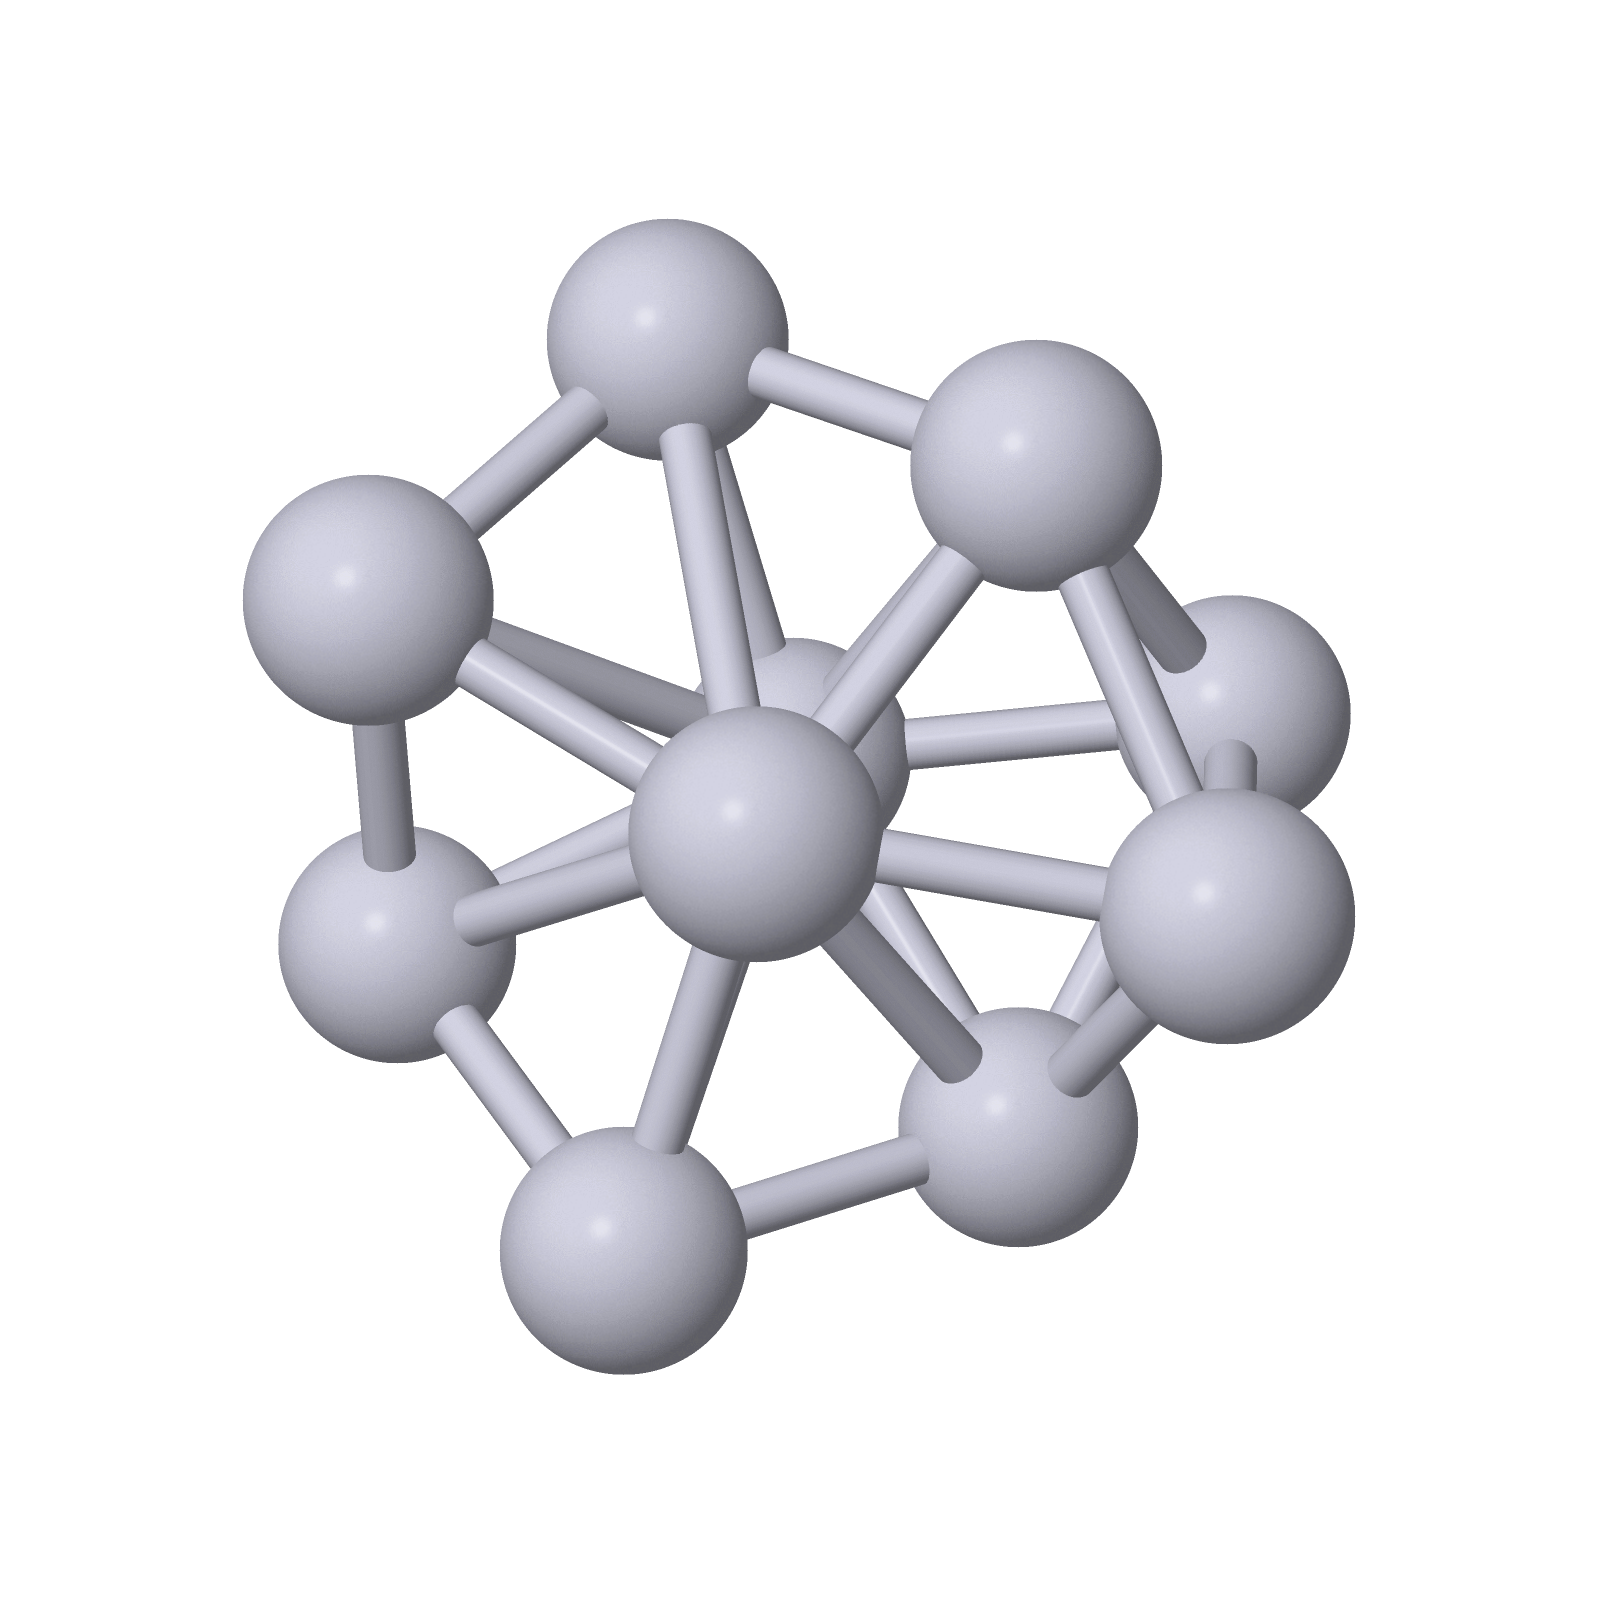
\includegraphics[width=\imgw]{Pt10CO/pt10_ref.png}};
\node[inner sep=0pt] (pt6ge4cross) at (\rightx,\topy)
  {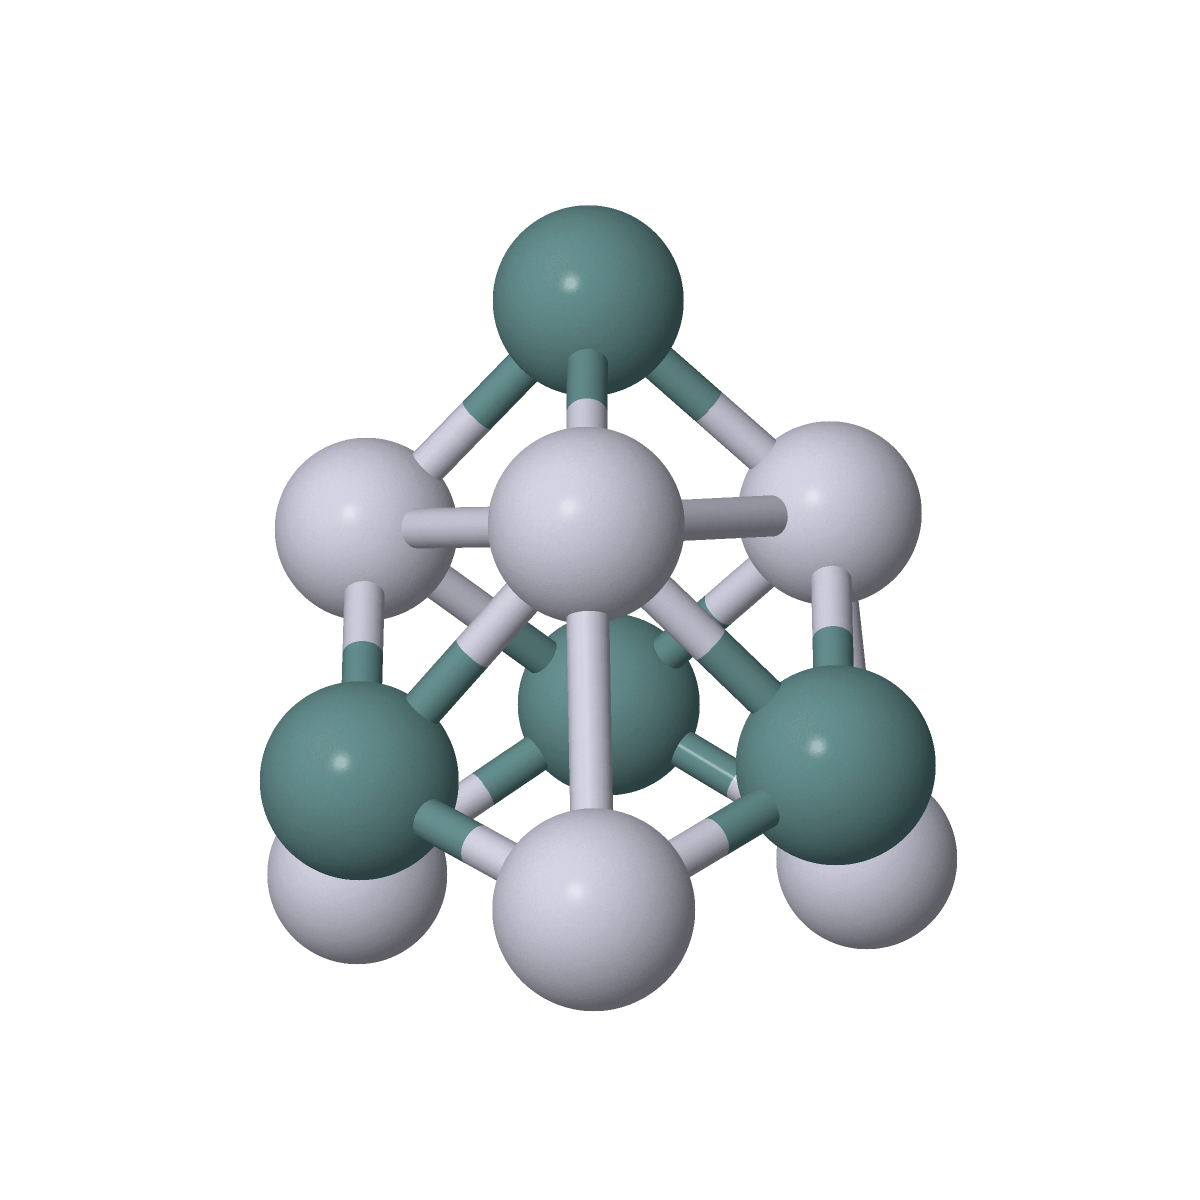
\includegraphics[width=\imgw]{pt6ge4.png}};
\node[inner sep=0pt] (pt5ge5cross) at (\leftx,\bottomy)
  {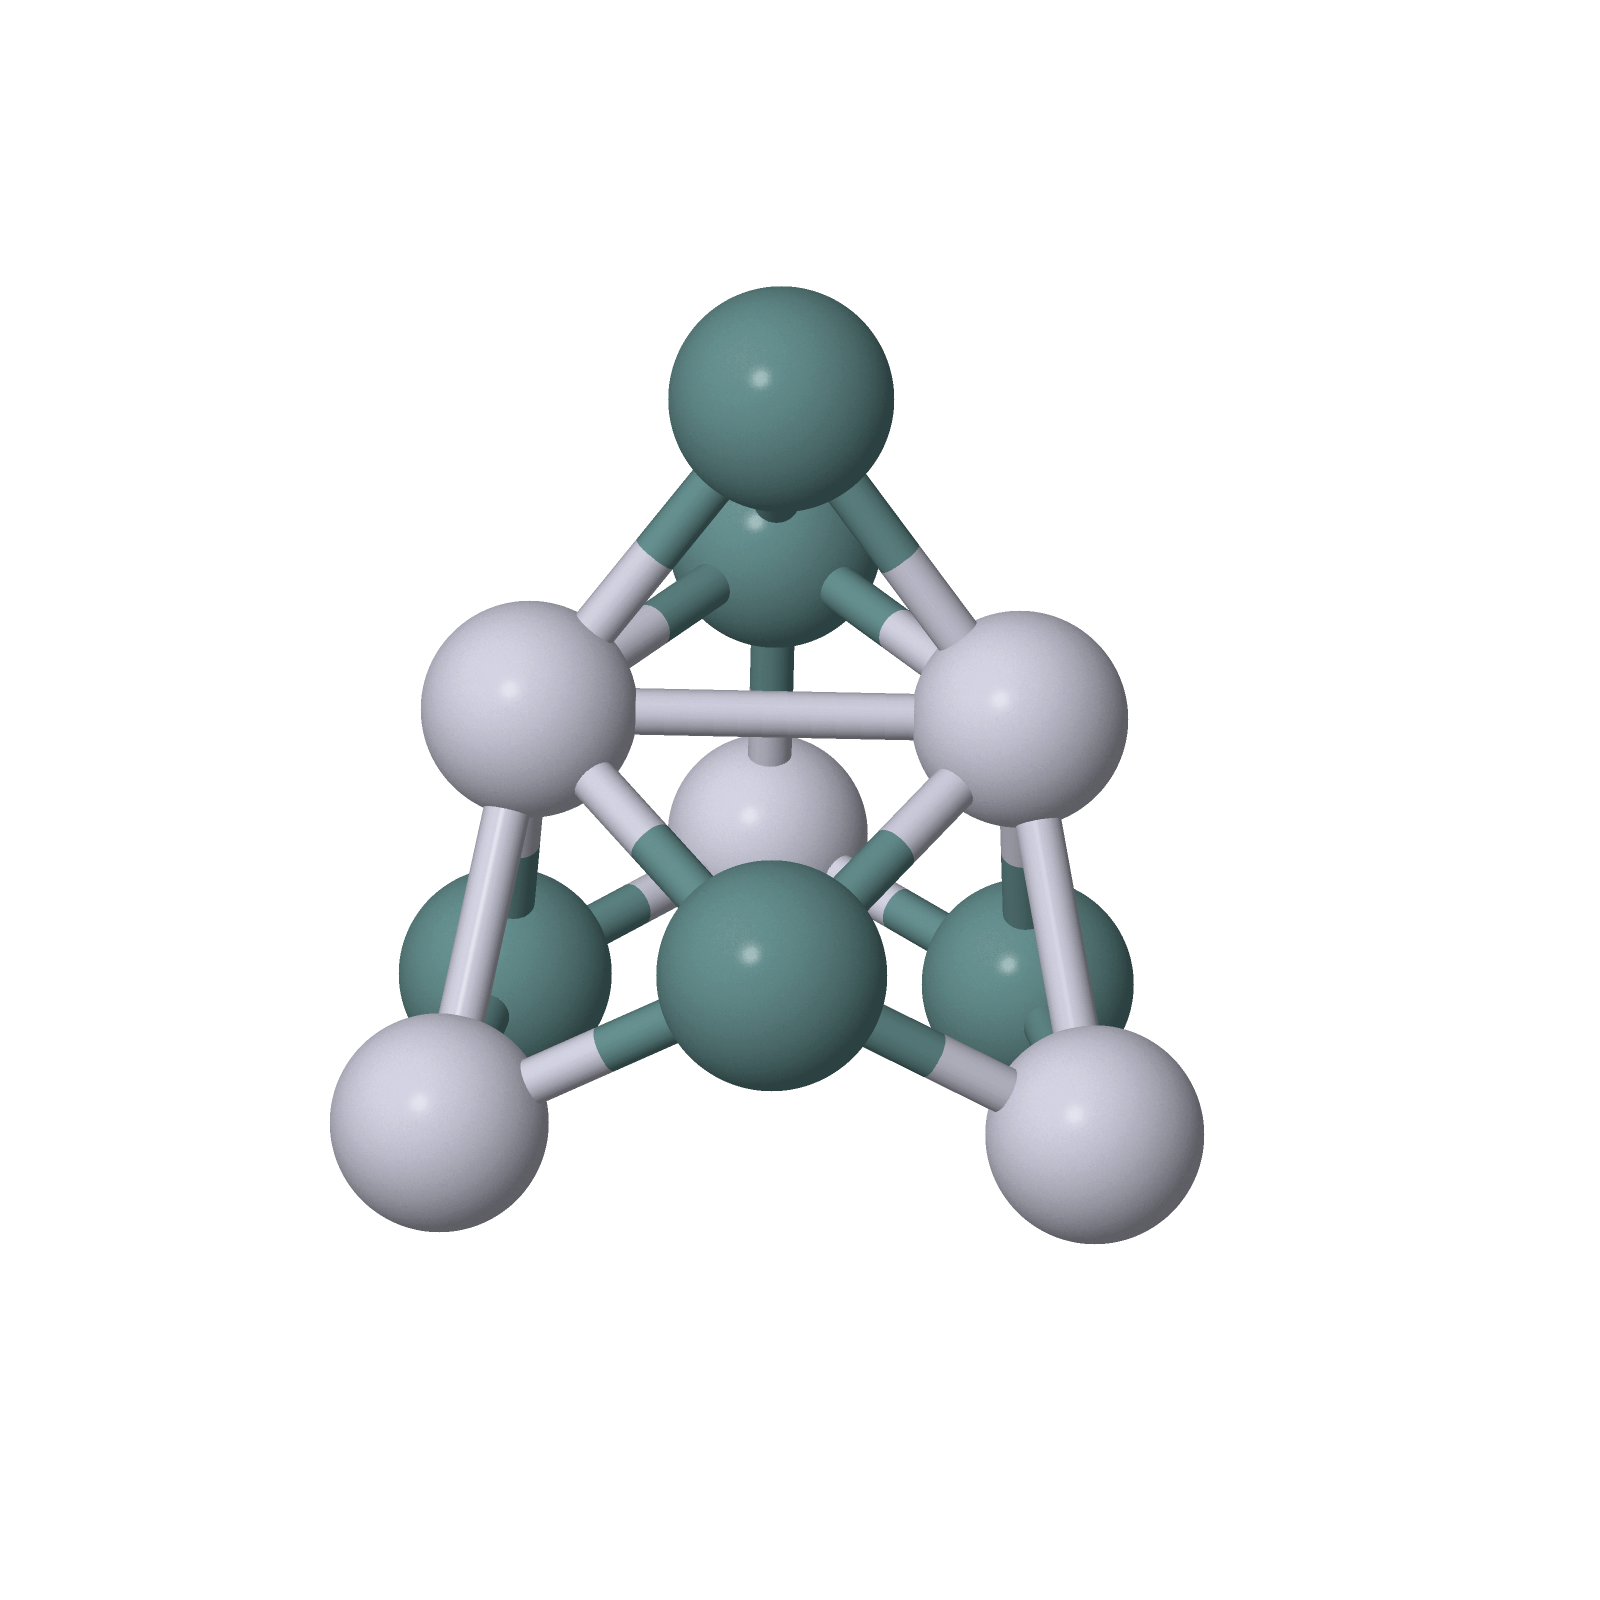
\includegraphics[width=\imgw]{Pt5Ge5_fromPt10Parent.png}};
\node[inner sep=0pt] (pt4ge6cross) at (\rightx,\bottomy)
  {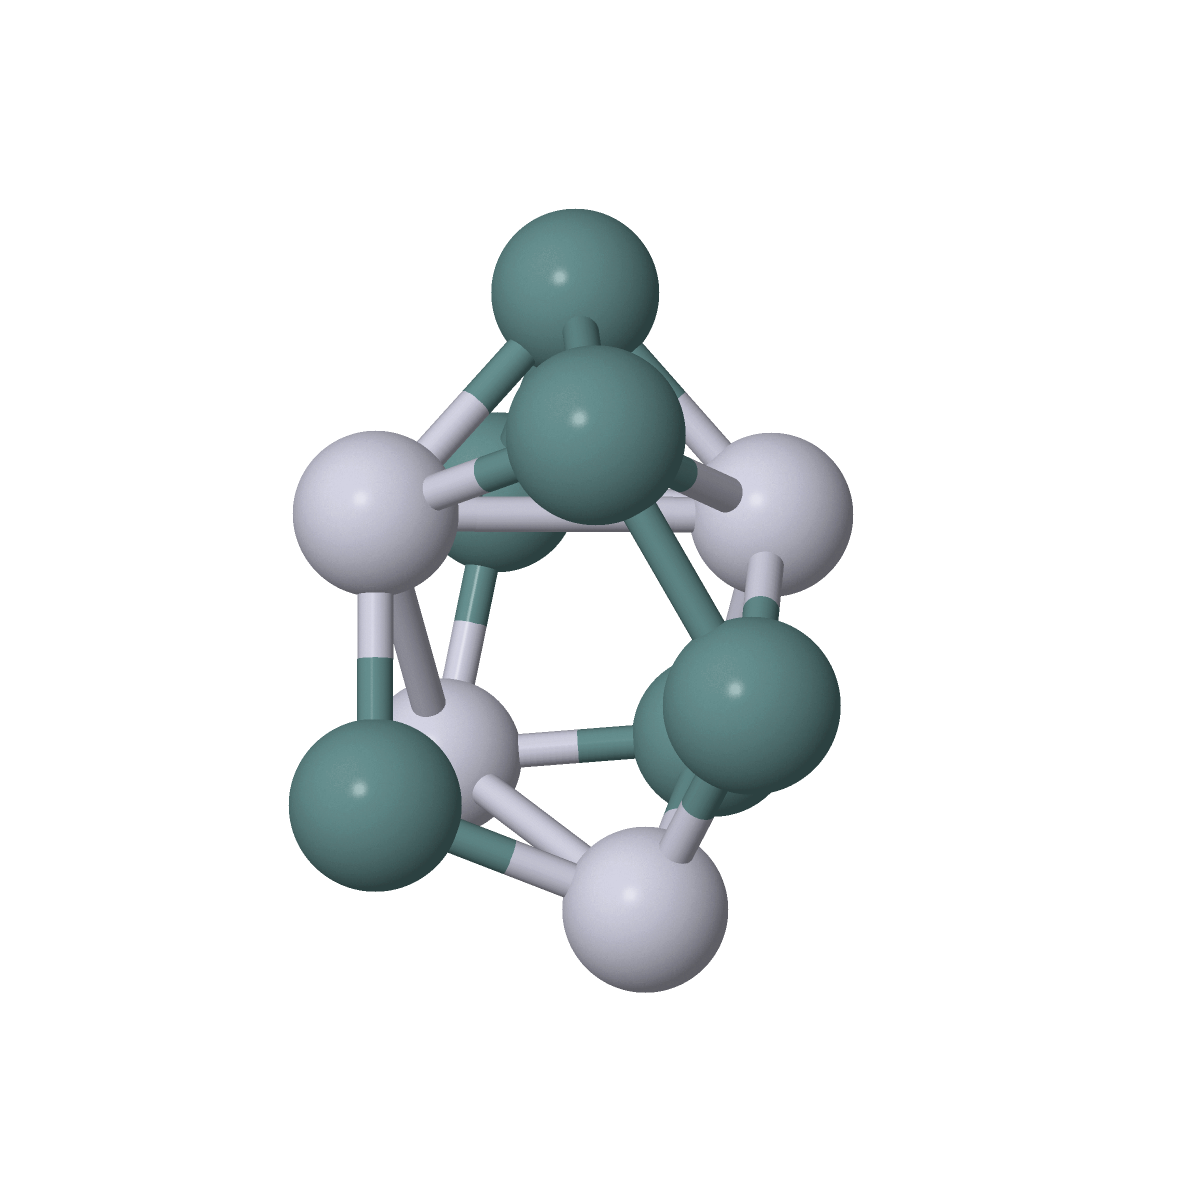
\includegraphics[width=\imgw]{pt4ge6.png}};

% Panel markers.
\node[panel] at ([xshift=-1.60cm,yshift=1.52cm]pt10cross.center) {(a)};
\node[panel] at ([xshift=-1.60cm,yshift=1.52cm]pt6ge4cross.center) {(b)};
\node[panel] at ([xshift=-1.60cm,yshift=1.52cm]pt5ge5cross.center) {(c)};
\node[panel] at ([xshift=-1.60cm,yshift=1.52cm]pt4ge6cross.center) {(d)};

% Model labels.
\node[title] at ([yshift=\titleshift]pt10cross.center)
  {\ce{Pt10^{der}}};
\node[title] at ([yshift=\titleshift]pt6ge4cross.center)
  {\ce{Pt6Ge4^{der}}};
\node[title] at ([yshift=\titleshift]pt5ge5cross.center)
  {\ce{Pt5Ge5^{der}}};
\node[title] at ([yshift=\titleshift]pt4ge6cross.center)
  {\ce{Pt4Ge6^{der}}};

% Pt10 site numbers.
\node[sitelabel] at ([xshift=-.10cm,yshift=-0.02cm]pt10cross.center) {1};
\node[sitelabel] at ([xshift=0.54cm,yshift=0.92cm]pt10cross.center) {3};
\node[sitelabel] at ([xshift=1.10cm,yshift=-0.25cm]pt10cross.center) {4};
\node[sitelabel] at ([xshift=1.12cm,yshift=0.30cm]pt10cross.center) {2};
\node[sitelabel] at ([xshift=-0.35cm,yshift=1.22cm]pt10cross.center) {10};
\node[sitelabel] at ([xshift=-1.12cm,yshift=0.58cm]pt10cross.center) {8};
\node[sitelabel] at ([xshift=-1.02cm,yshift=-0.33cm]pt10cross.center) {7};
\node[sitelabel] at ([xshift=-.5cm,yshift=-1.10cm]pt10cross.center) {6};
\node[sitelabel] at ([xshift=.58cm,yshift=-0.82cm]pt10cross.center) {5};
\node[sitelabel] at ([xshift=.12cm,yshift=.57cm]pt10cross.center) {9};

% Pt6Ge4 representative adsorption-site classes. Positions are tied to the
% selected Jmol view and can be fine-tuned independently.
\node[sitelabel] at ([xshift=-0.83cm,yshift=0.30cm]pt6ge4cross.center) {1};
\node[sitelabel] at ([xshift=-0.03cm,yshift=0.27cm]pt6ge4cross.center) {2};
\node[sitelabel] at ([xshift=0.82cm,yshift=0.32cm]pt6ge4cross.center) {4};
\node[sitelabel] at ([xshift=-0.02cm,yshift=-1.05cm]pt6ge4cross.center) {9};
\node[sitelabel] at ([xshift=-0.92cm,yshift=-1.26cm]pt6ge4cross.center) {7};
\node[sitelabel] at ([xshift=1.02cm,yshift=-1.26cm]pt6ge4cross.center) {5};

% Pt5Ge5 site-class numbers.
\node[sitelabel] at ([xshift=-.72cm,yshift=.30cm]pt5ge5cross.center) {6};
\node[sitelabel] at ([xshift=.60cm,yshift=.30cm]pt5ge5cross.center) {8};
\node[sitelabel] at ([xshift=-0.1cm,yshift=0.0cm]pt5ge5cross.center) {4};
\node[sitelabel] at ([xshift=-0.92cm,yshift=-0.78cm]pt5ge5cross.center) {7};
\node[sitelabel] at ([xshift=0.72cm,yshift=-0.78cm]pt5ge5cross.center) {10};

% Pt4Ge6 adsorption sites.
\node[sitelabel] at ([xshift=-0.75cm,yshift=0.34cm]pt4ge6cross.center) {1};
\node[sitelabel] at ([xshift=0.58cm,yshift=0.34cm]pt4ge6cross.center) {2};
\node[sitelabel] at ([xshift=-0.42cm,yshift=-0.46cm]pt4ge6cross.center) {5};
\node[sitelabel] at ([xshift=0.14cm,yshift=-1.0cm]pt4ge6cross.center) {7};

\end{tikzpicture}

\end{adjustbox}
\caption{Numbering of the Pt atoms used to place \ce{CO} and calculate the
\ce{CO} binding energies. Panel (a) shows \ce{Pt10^{der}}. Panels (b)--(d)
show the \ce{Pt6Ge4^{der}}, \ce{Pt5Ge5^{der}}, and \ce{Pt4Ge6^{der}} models obtained from
\ce{Pt10^{GM}}, respectively. The labels retain the Pt-atom numbering of each derivative
starting structure; the GM structures use consecutive Pt numbering within
each composition.}
\label{fig:tfg_site_numbering}
\end{figure}

\begin{table}[htbp]
\caption{Hoppe ECoN values for each Pt atom in the two optimized \ce{Pt10}
structures compared in Section~3.2. Only Pt neighbors are included. The
\ce{Pt10^{GM}} structure is a nonet, whereas \ce{Pt10^{der}} is a triplet.
The \ce{Pt10^{der}} values use the selected orbital-stable
triplet geometry. Atom numbers refer to the bare-cluster geometries; the
corresponding adsorption-site labels for \ce{Pt10^{der}} are given in
Supporting Table~\ref{tab:tfg_pt10_der_econ_co}.}
\label{tab:tfg_pt10_bare_econ}
\begin{adjustbox}{max width=\linewidth}
\begin{tabular}{ccc}
\toprule
{Pt atom} & {\ce{Pt10^{GM}} nonet} & {\ce{Pt10^{der}} triplet} \\
\midrule
1  & 5.69 & 3.03 \\
2  & 5.69 & {4.54} \\
3  & 5.69 & {5.94} \\
4  & 3.00 & {3.16} \\
5  & 3.00 & 3.95 \\
6  & 5.69 & {5.94} \\
7  & 3.00 & {3.95} \\
8  & 5.68 & {3.03} \\
9  & 5.68 & {3.16} \\
10 & 3.00 & {4.55} \\
\bottomrule
\end{tabular}
\end{adjustbox}
\end{table}

\begin{table}[htbp]
%\color{ForestGreen}
\centering
\caption{Initial and final local ECoN values for the triplet
\ce{Pt10^{der}} adsorption series. Initial values use the selected
orbital-stable bare-cluster geometry. Final values refer to the Pt atom
bound to \ce{CO} in each optimized carbonyl. Only Pt neighbors are included.
Site labels identify the initial adsorption positions; the Pt atom column
gives the corresponding atom number in the bare-cluster reference of
Supporting Table~\ref{tab:tfg_pt10_bare_econ}.
$\Delta ECoN=ECoN^{\ce{CO}}-ECoN^{0}$ is calculated before rounding.}
\label{tab:tfg_pt10_der_econ_co}
\small
\begin{adjustbox}{max width=\linewidth}
\begin{tabular}{cccccc}
\toprule
{Site} & {Pt atom} & {$ECoN^{0}$} & {$ECoN^{\ce{CO}}$} &
{$\Delta ECoN$} & {$BE_{\rm ad}(\ce{CO})$ / eV} \\
\midrule
1  & 6  & 5.94 & 5.69 & -0.25 & -2.16 \\
2  & 10 & 4.55 & 3.00 & -1.54 & -2.49 \\
3  & 7  & 3.95 & 3.98 & 0.03 & -2.59 \\
4  & 5  & 3.95 & 3.97 & 0.02 & -2.58 \\
5  & 1  & 3.03 & 3.98 & 0.95 & -2.59 \\
6  & 9  & 3.16 & 3.96 & 0.80 & -2.66 \\
7  & 4  & 3.16 & 4.06 & 0.90 & -2.49 \\
8  & 8  & 3.03 & 4.97 & 1.94 & -2.65 \\
9  & 3  & 5.94 & 5.69 & -0.25 & -2.16 \\
10 & 2  & 4.54 & 4.97 & 0.43 & -2.65 \\
\bottomrule
\end{tabular}
\end{adjustbox}
\end{table}

\subsection*{AdNDP analysis}

The previously reported AdNDP analysis of \ce{Pt10^{GM}} identified 30
1c lone-pair elements (ON = $1.83|e|$), 16 3c--2e elements on the external
triangular faces (ON = $1.97|e|$), four 3c--1e elements on the internal
triangular faces (ON = $0.99|e|$), and four 4c--1e elements (ON =
$0.93|e|$). For \ce{Pt5Ge5^{GM}}, the reported analysis found 15 Pt-centered
1c--2e elements (ON = $1.84|e|$) and 20 Pt--Ge 2c--2e elements (ON =
$1.86|e|$)\cite{ugartemendia:2022}.

\begin{table}[htbp]
\caption{Summary of the AdNDP decompositions for the derivative models.
The \ce{Pt5Ge5} row reports model E. For rows with several element types,
the ON ranges follow the same order as the listed elements. ON denotes the
AdNDP occupation number.
For the triplet \ce{Pt10}, the alpha and beta density matrices were analyzed
independently. The 3c elements involving the same atomic centers in both spin
components were paired to obtain their combined occupations.}
\label{tab:tfg_adndp_summary}
\renewcommand{\arraystretch}{1.08}
\setlength{\tabcolsep}{2.8pt}
\small
\begin{adjustbox}{max width=\linewidth}
\begin{tabular}{@{}>{\raggedright\arraybackslash}p{1.25cm}
                 >{\raggedright\arraybackslash}p{1.55cm}
                 >{\raggedright\arraybackslash}p{5.25cm}
                 >{\raggedright\arraybackslash}p{3.75cm}
                 >{\raggedright\arraybackslash}p{2.75cm}@{}}
\toprule
 & {$2S+1$} & {AdNDP elements} & {ON range} & {Interpretation} \\
\midrule
			\ce{Pt10} & 3 & \begin{tabular}[t]{@{}l@{}}
			\(\alpha\): 30 $\times$ Pt-centered 1c\\
			\hspace{.3cm}21 $\times$ Pt 3c\\
			\(\beta\): 30 $\times$ Pt-centered 1c\\
			\hspace{.3cm}19 $\times$ Pt 3c
			\end{tabular} & \begin{tabular}[t]{@{}l@{}}
			\(\alpha\): 0.967--0.992 (1c)\\
			\hspace{.3cm}0.990--0.997 (3c)\\
			\(\beta\): 0.961--0.989 (1c)\\
			\hspace{.3cm}0.994--0.997 (3c)\\
			paired 3c: 1.984--1.994
			\end{tabular} & \begin{tabular}[t]{@{}l@{}}19 $\times$ 3c--2e\\
		2 $\times$ 3c--1e;\\delocalized\\multicenter model\end{tabular} \\\hline
\ce{Pt5Ge5} & 1 & \begin{tabular}[t]{@{}l@{}}20 $\times$ Pt-centered 1c--2e\\14
	$\times$ Pt--Ge 2c--2e\\3 $\times$ Pt--Pt 2c--2e\end{tabular} &
	\begin{tabular}[t]{@{}l@{}}1.820--1.970\\1.842--1.983\\1.873--1.905\end{tabular}
			& localized 1c and 2c bonding \\\hline
\ce{Pt6Ge4} & 1 & \begin{tabular}[t]{@{}l@{}}12 $\times$ Pt-centered 1c--2e\\5 $\times$ Pt--Pt 2c--2e\\21 $\times$ Pt--Ge 2c--2e\end{tabular} & \begin{tabular}[t]{@{}l@{}}1.916--1.968\\1.975--1.983\\1.894--1.982\end{tabular} & localized Pt--Pt/Pt--Ge bonding \\\hline
\ce{Pt4Ge6} & 1 & \begin{tabular}[t]{@{}l@{}}12 $\times$ Pt-centered 1c--2e\\2 $\times$ Pt--Pt 2c--2e\\15 $\times$ Pt--Ge 2c--2e\\3 $\times$ Ge--Ge 2c--2e\end{tabular} & \begin{tabular}[t]{@{}l@{}}1.841--1.978\\1.903--1.919\\1.865--1.977\\1.813--1.861\end{tabular} & localized one- and two-center bonding \\
			\bottomrule
\end{tabular}
\end{adjustbox}
\parbox{0.96\linewidth}{\footnotesize For \ce{Pt10}, the listed occupations
refer to individual spin channels and are therefore close to one. The residual
alpha and beta densities are 0.713 and 0.873 electrons, respectively. The
threshold parameter was 1.040 for the 1c and 3c searches, corresponding to a
minimum accepted spin-resolved ON of 0.960. Nineteen alpha and beta 3c
elements involve identical sets of Pt atoms; their summed occupations are
listed as paired 3c values. The remaining alpha 3c elements are located on
Pt(2)--Pt(3)--Pt(7) and Pt(5)--Pt(6)--Pt(10), with ON values of 0.994 and
0.995, respectively. For the \ce{Pt5Ge5} model E decomposition, the 1c and
2c thresholds were both 0.180; the residual density was 0.016 electrons.
The 1c--2e and 2c--2e labels identify the AdNDP element types; the actual
occupations are the ON values listed in the table and are not exactly two.
The 1c and 2c parameters were 0.100 and 0.140 for \ce{Pt6Ge4},
and 0.160 and 0.250 for \ce{Pt4Ge6}.}
\end{table}

\begin{table}[htbp]
\caption{Binding energies for \ce{CO} placed at different Pt atoms, together
with structural and vibrational descriptors, for carbonyls initiated from the
reported global-minimum (GM) structures. The multiplicity is that of the corresponding bare-cluster
GM: triplet for \ce{Pt6Ge4} and singlet for \ce{Pt5Ge5} and \ce{Pt4Ge6}. Each
$BE_{\rm ad}(\ce{CO})$ uses free singlet \ce{CO} and the
corresponding bare GM cluster with the same multiplicity.
Site labels follow consecutive Pt numbering
within each GM cluster. Grouped labels denote initial sites represented by
the same optimized carbonyl.}
The same labels are used in Supporting
Tables~\ref{tab:tfg_gm_ptge_econ_pre_descriptors} and
\ref{tab:tfg_gm_ptge_econ_descriptors}.
\label{tab:tfg_gm_bimetallic_adsorption_descriptors}
%\scriptsize
\begin{adjustbox}{max width=\linewidth}
\begin{tabular}{lccccc}
\toprule
{Composition} & {Site} & {$BE_{\rm ad}(\ce{CO})$ / eV} &
{$r(\ce{Pt-C})$ / \AA} & {$r(\ce{C-O})$ / \AA} &
{$\nu(\ce{CO})$ / \si{\per\centi\metre}} \\
\midrule
\ce{Pt6Ge4^{GM}CO} & 2 & -1.95 & 1.85 & 1.16 & 2019 \\
\ce{Pt6Ge4^{GM}CO} & 6 & -1.84 & 1.85 & 1.16 & 2023 \\
\ce{Pt6Ge4^{GM}CO} & 3 & -1.73 & 1.86 & 1.16 & 2017 \\
\ce{Pt6Ge4^{GM}CO} & 1 & -1.66 & 1.85 & 1.16 & 2022 \\
\ce{Pt6Ge4^{GM}CO} & 5 & -1.22 & 1.93 & 1.15 & 2011 \\
\ce{Pt6Ge4^{GM}CO} & 4 & -1.21 & 1.91 & 1.16 & 2014 \\
\midrule
\ce{Pt5Ge5^{GM}CO} & 1/2/4/5 & -1.35 & 1.90 & 1.16 & 2006 \\
\ce{Pt5Ge5^{GM}CO} & 3 & -0.79 & 1.96 & 1.15 & 2022 \\
\midrule
\ce{Pt4Ge6^{GM}CO} & 2 & -1.51 & 1.91 & 1.16 & 2010 \\
\ce{Pt4Ge6^{GM}CO} & 4 & -1.24 & 1.93 & 1.15 & 2012 \\
\ce{Pt4Ge6^{GM}CO} & 1 & -1.15 & 1.92 & 1.16 & 2007 \\
\ce{Pt4Ge6^{GM}CO} & 3 & -1.05 & 1.92 & 1.16 & 2003 \\
\bottomrule
\end{tabular}
\end{adjustbox}
\end{table}

\begin{table}[htbp]
\caption{Pre-adsorption local Hoppe ECoN descriptors for the Pt sites in the
optimized global-minimum (GM) Pt--Ge clusters. Only metal neighbors
are included, with
$ECoN_{\rm total}^{0}=ECoN_{\rm Pt}^{0}+ECoN_{\rm Ge}^{0}$ and
$x_{\rm Ge}^{0}=ECoN_{\rm Ge}^{0}/ECoN_{\rm total}^{0}$. The binding
energies correspond to carbonyls with the spin state of the corresponding
bare-cluster GM. \protect{The GM is a triplet for \ce{Pt6Ge4} and a singlet for
\ce{Pt5Ge5} and \ce{Pt4Ge6}.}
Site labels follow the consecutive Pt numbering used for
the GM binding energies in Supporting
Table~\ref{tab:tfg_gm_bimetallic_adsorption_descriptors}.}
\label{tab:tfg_gm_ptge_econ_pre_descriptors}
\small
\begin{adjustbox}{max width=\linewidth}
\begin{tabular}{lccrrrr}
\toprule
{System} & {Site} & {$BE_{\rm ad}(\ce{CO})$ / eV} &
{$ECoN_{\rm total}^{0}$} & {$ECoN_{\rm Pt}^{0}$} &
{$ECoN_{\rm Ge}^{0}$} & {$x_{\rm Ge}^{0}$} \\
\midrule
\ce{Pt6Ge4^{GM}CO} & 2 & -1.95 & 3.84 & 2.55 & 1.29 & 0.34 \\
\ce{Pt6Ge4^{GM}CO} & 3 & -1.73 & 3.96 & 1.73 & 2.23 & 0.56 \\
\ce{Pt6Ge4^{GM}CO} & 1 & -1.66 & 4.87 & 2.57 & 2.30 & 0.47 \\
\ce{Pt6Ge4^{GM}CO} & 6 & -1.84 & 3.95 & 1.75 & 2.20 & 0.56 \\
\ce{Pt6Ge4^{GM}CO} & 5 & -1.22 & 3.89 & 0.77 & 3.12 & 0.80 \\
\ce{Pt6Ge4^{GM}CO} & 4 & -1.21 & 3.87 & 0.75 & 3.12 & 0.81 \\
\midrule
\ce{Pt5Ge5^{GM}CO} &  1/2/4/5 & -1.35 & 3.48 & 0.24 & 3.24 & 0.93 \\
\ce{Pt5Ge5^{GM}CO} & 3 & -0.79 & 4.03 & 0.01 & 4.02 & 1.00 \\
\midrule
\ce{Pt4Ge6^{GM}CO} & 2 & -1.51 & 4.61 & 0.37 & 4.24 & 0.92 \\
\ce{Pt4Ge6^{GM}CO} & 4 & -1.24 & 3.02 & 0.00 & 3.01 & 1.00 \\
\ce{Pt4Ge6^{GM}CO} & 1 & -1.15 & 2.99 & 0.00 & 2.99 & 1.00 \\
\ce{Pt4Ge6^{GM}CO} & 3 & -1.05 & 4.71 & 0.45 & 4.26 & 0.91 \\
\bottomrule
\end{tabular}
\end{adjustbox}
\end{table}

\begin{table}[htbp]
\caption{Local Hoppe ECoN descriptors for the Pt atom bound to \ce{CO} in
the optimized atom-substitution Pt--Ge carbonyls. The superscript \ce{CO}
distinguishes these final-state descriptors from the pre-adsorption values in
Table~\ref{tab:tfg_crossed_ptge_econ_descriptors}.
Site labels retain the derivative-model indices shown in
Supporting Figure~\ref{fig:tfg_site_numbering}, matching the pre-adsorption
labels in Table~\ref{tab:tfg_crossed_ptge_econ_descriptors}. Only metal neighbors are
included, with
$ECoN_{\rm total}^{\ce{CO}}=ECoN_{\rm Pt}^{\ce{CO}}+ECoN_{\rm Ge}^{\ce{CO}}$
and
$x_{\rm Ge}^{\ce{CO}}=ECoN_{\rm Ge}^{\ce{CO}}/ECoN_{\rm total}^{\ce{CO}}$.}
\label{tab:tfg_crossed_ptge_econ_co_descriptors}
\small
\begin{adjustbox}{max width=\linewidth}
\begin{tabular}{lcrrrrr}
\toprule
{System} & {Site} & {$BE_{\rm ad}(\ce{CO})$ / eV} &
{$ECoN_{\rm total}^{\ce{CO}}$} & {$ECoN_{\rm Pt}^{\ce{CO}}$} &
{$ECoN_{\rm Ge}^{\ce{CO}}$} & {$x_{\rm Ge}^{\ce{CO}}$} \\
\midrule
\ce{Pt6Ge4^{der}CO}  & 2   & -2.25 & 3.00 & 1.77 & 1.23 & 0.41 \\
\ce{Pt6Ge4^{der}CO}  & 9   & -2.25 & 3.01 & 1.16 & 1.85 & 0.61 \\
\ce{Pt6Ge4^{der}CO}  & 1/4 & -2.24 & 4.30 & 2.43 & 1.88 & 0.44 \\
\ce{Pt6Ge4^{der}CO}  & 5/7 & -1.57 & 2.87 & 0.66 & 2.22 & 0.77 \\
\midrule
\ce{Pt5Ge5^{der}CO}  & 6/8  & -2.08 & 5.69 & 1.69 & 4.00 & 0.70 \\
\ce{Pt5Ge5^{der}CO}  & 7/10 & -1.66 & 2.95 & 0.94 & 2.02 & 0.68 \\
\ce{Pt5Ge5^{der}CO}  & 4    & -1.34 & 2.98 & 0.00 & 2.98 & 1.00 \\
\midrule
\ce{Pt4Ge6^{der}CO}  & 5/7 & -1.46 & 3.92 & 0.69 & 3.23 & 0.83 \\
\ce{Pt4Ge6^{der}CO}  & 2   & -1.31 & 3.22 & 0.13 & 3.09 & 0.96 \\
\ce{Pt4Ge6^{der}CO}  & 1   & -1.05 & 5.90 & 1.42 & 4.48 & 0.76 \\
\bottomrule
\end{tabular}
\end{adjustbox}
\end{table}

\begin{table}[htbp]
\caption{Local Hoppe ECoN descriptors for the Pt atom bound to \ce{CO} in
the optimized GM Pt--Ge carbonyls. Each composition is represented
using the spin state of its bare-cluster GM. The GM is a triplet for
\ce{Pt6Ge4} and a singlet for \ce{Pt5Ge5} and \ce{Pt4Ge6}. The superscript \ce{CO} indicates that these
descriptors are evaluated after adsorption and relaxation.
Site labels follow the same consecutive Pt numbering as the
pre-adsorption GM descriptors in Supporting
Table~\ref{tab:tfg_gm_ptge_econ_pre_descriptors}.}
\label{tab:tfg_gm_ptge_econ_descriptors}
%\scriptsize
\begin{adjustbox}{max width=\linewidth}
\begin{tabular}{llrrrrr}
\toprule
{System} & {Site} & {$BE_{\rm ad}(\ce{CO})$ / eV} &
{$ECoN_{\rm total}^{\ce{CO}}$} & {$ECoN_{\rm Pt}^{\ce{CO}}$} &
{$ECoN_{\rm Ge}^{\ce{CO}}$} & {$x_{\rm Ge}^{\ce{CO}}$} \\
\midrule
\ce{Pt6Ge4^{GM}CO} & 2  & -1.95 & 3.97 & 2.85 & 1.12 & 0.28 \\
\ce{Pt6Ge4^{GM}CO} & 6  & -1.84 & 4.28 & 2.35 & 1.93 & 0.45 \\
\ce{Pt6Ge4^{GM}CO} & 3  & -1.73 & 4.10 & 2.15 & 1.95 & 0.48 \\
\ce{Pt6Ge4^{GM}CO} & 1  & -1.66 & 5.08 & 3.03 & 2.04 & 0.40 \\
\ce{Pt6Ge4^{GM}CO} & 5  & -1.22 & 3.92 & 0.90 & 3.02 & 0.77 \\
\ce{Pt6Ge4^{GM}CO} & 4  & -1.21 & 2.93 & 0.77 & 2.16 & 0.74 \\
\midrule
\ce{Pt5Ge5^{GM}CO} & 1/2/4/5  & -1.35 & 4.52 & 1.55 & 2.98 & 0.66 \\
\ce{Pt5Ge5^{GM}CO} & 3  & -0.79 & 3.96 & 0.01 & 3.96 & 1.00 \\
\midrule
\ce{Pt4Ge6^{GM}CO} & 2  & -1.51 & 4.61 & 0.41 & 4.20 & 0.91 \\
\ce{Pt4Ge6^{GM}CO} & 4  & -1.24 & 2.97 & 0.00 & 2.97 & 1.00 \\
\ce{Pt4Ge6^{GM}CO} & 1  & -1.15 & 4.08 & 0.22 & 3.86 & 0.95 \\
\ce{Pt4Ge6^{GM}CO} & 3  & -1.05 & 4.71 & 0.55 & 4.16 & 0.88 \\
\bottomrule
\end{tabular}
\end{adjustbox}
\end{table}


\clearpage
\bibliography{refs,bib}

\end{document}
